\documentclass[12pt]{article}
\usepackage{./util/settings}
\usepackage{graphicx,url}
\usepackage[utf8]{inputenc}
\usepackage[brazil]{babel}
\usepackage{tikz}
     
\sloppy

\title{Heurística de Roteamento e Alocação de Fibras em Redes Ópticas}

\author{Diego M. A. Lütke}


\address{Escola Politécnica -- Pontifícia Universidade Católica do Paraná (PUCPR)
	\email{diegolutke@hotmail.com}
}


\begin{document}
\maketitle

\begin{resumo} 
  O presente artigo desenvolve um algoritmo heurístico de roteamento em redes
  ópticas para encontrar o caminho físico entre dois pontos ($A$ e $B$). A proposta
  utiliza o algoritmo de Dijkstra aplicado a uma topologia de rede óptica
  modelada como grafo. São discutidos elementos constituintes das redes
  ópticas, alternativas de algoritmos de roteamento, e aspectos de complexidade
  relacionados à programação linear e problemas NP-difíceis.
\end{resumo}

\section{Introdução}

Atualmente, as redes ópticas representam a espinha dorsal da conectividade
global, responsáveis pela transmissão de grandes volumes de dados em torno do
globo terrestre via cabos terrestres e submarinos. Embora as normas e os desafios
iniciais das implementações de redes ópticas pioneiras tenham atigindo um platô
de estabilidade na última década devido a expansão desse tipo de rede dos
backbones para as redes de acesso, ainda há uma série de desafios relacionados
a operação e manutenção desse tipo de rede.

Um desses desafios é o roteamento de caminhos físicos, isto é, a definição de
quais fibras ópticas devem ser utilizadas para interligar dois pontos de
acesso. Este artigo propõe desenvolver um algoritmo heurístico para o
roteamento de uma fibra dado uma rede em funcionamento. Para isso, o artigo é
estruturado da seguinte forma: na Seção \ref{sec:fundaments} aborda-se os
elementos de rede relevantes para o estudo proposto, os algoritmos de base e o
que já existe de estudos acadêmicos relevantes próximo do presente artigo na
Seção \ref{sec:problem} define-se e delimita-se o problema de roteamento, na
Seção \ref{sec:algorithm} desenvolve-se o algoritmo e, por fim, as
considerações finais são dadas em \ref{sec:conclusion}.


\section{Fundamentação Teórica} \label{sec:fundaments}

Para o roteamento de fibras, é necessário pelo menos o entendimento básico de
dois temas: (1) a composição de elementos passivos das redes ópticas e (2)
algoritmos (no sentido de operações, otimização e tipos de problemas).

\subsection{Redes Ópticas}

Na teoria dos grafos, um grafo é uma estrutura composta por vértices ($V$)
(também chamados de nós) e arestas ($E$). A relação entre $V$ e $E$ é dado por
$G(V,E)$. Fazendo um paralelo com uma rede óptica, os vértices seriam as Caixas
de Emenda (CE) e as Caixas de Atendimento (CA) \cite{maeda2009optical}; os
cabos ópticos por sua vez seriam as arestas. Um exemplo de CE poste ser visto
na Figura \ref{fig:ce_fixacao_poste}, a Figura \ref{fig:ce_detalhe_bandejas}
mostra o interior de uma CE.

Os cabos ópticos são constituídos de fibras agrupadas em tubos. Cada fibra por
sua vez, pode trafegar zero, um ou vários comprimentos de onda ($\lambda$).
Em uma rede física, as fibras são redirecionadas nos vértices (CEs e CAs) de
acordo com as demandas de atendimento das operadoras. CAs atendem clientes finais,
geralmente com o uso de tecnologias de Redes Ópticas Passivas (PON).

Esse redirecionamento das fibras ocorre com o uso de máquinas de fusão
\cite{maeda2009optical}, cada par de fibras é acomodado em bandejas, conforme
mostra a Figura \ref{fig:ce_detalhe_bandejas}. Em um caso ideal, espera-se que
de acordo com as requisições de demanda recebida, a ocupaćão das ranhuras seja
feita de forma sequencial e organizada. Por exemplo, em um cabo contendo 12
tubos, com 12 fibras cada cabo, o grupo de ranhuras superior recebe o primeiro
tubo, o segundo grupo o segundo tubo, assim por diante.

\begin{figure}
  \begin{minipage}[c]{0.43\linewidth}
	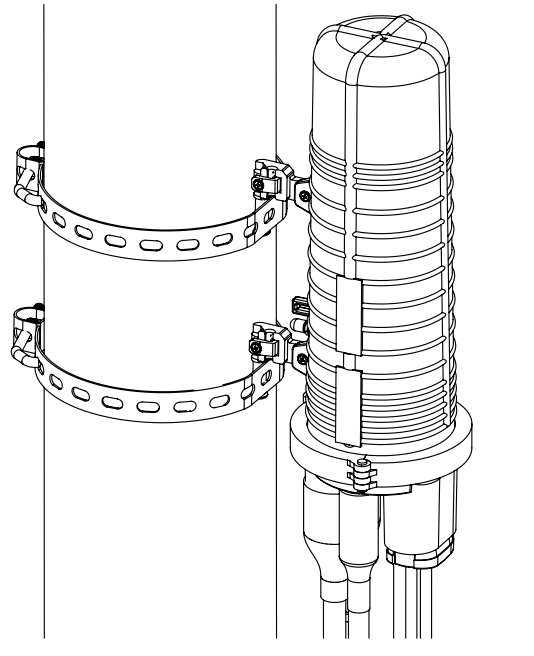
\includegraphics[width=\linewidth]{./images/caixa_emenda_fixacao_em_poste.png}
	\caption{CE fixada em poste}
	\label{fig:ce_fixacao_poste}
  \end{minipage}
  \hfill
  \begin{minipage}[c]{0.6\linewidth}
	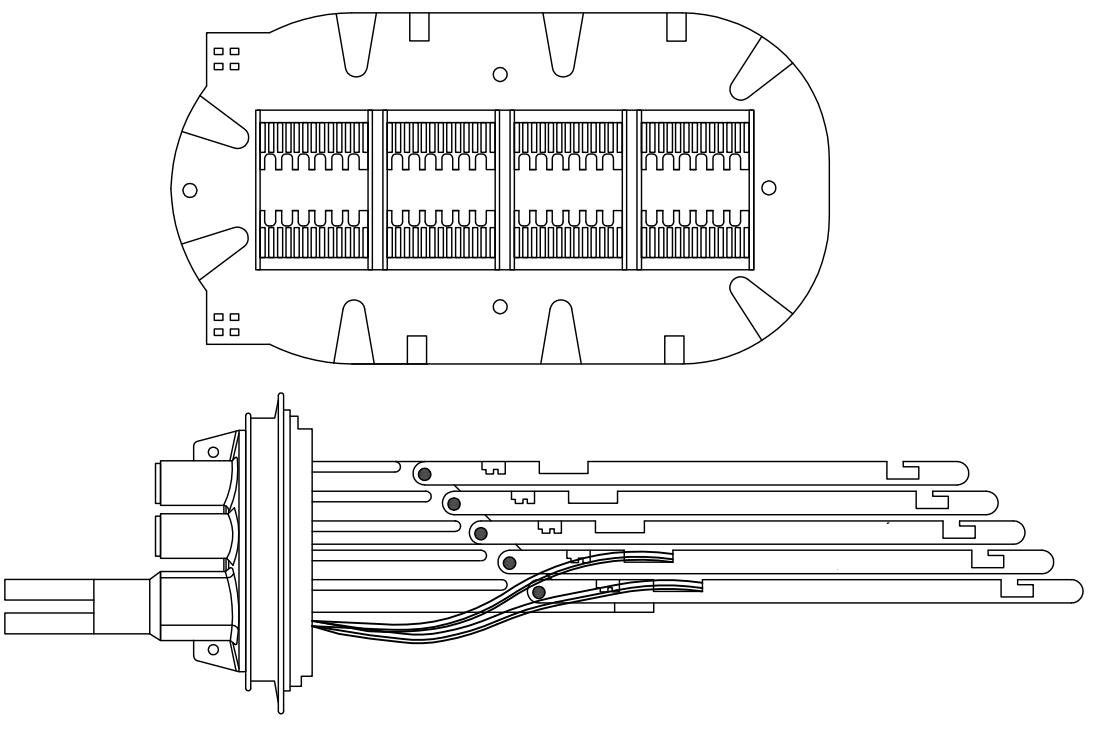
\includegraphics[width=\linewidth]{./images/caixa_emenda_detalhe_bandejas.png}
	\caption{Detalhe das bandejas de CE}
	\label{fig:ce_detalhe_bandejas}
  \end{minipage}
\end{figure}

\subsection{Algoritmos}

Para descobrir a melhor rota, ou seja, qual sequência de cabos e caixas é o 
caminho mais curto entre uma caixa A e B, podemos considerar pelo menos dois
algoritmos: Algoritmo de Dijkstra (encontra o caminho de menor custo em grafos
com pesos não negativos) \cite{dijkstra2022note} e o Algoritmo de Bellman-Ford
(lida com arestas de peso negativo, mas com maior complexidade temporal).

Embora o Algoritmo de Dijkstra não funcione com custos negativos, podemos
considerá-lo, visto que o custo será igual a distância, um exemplo de uso pode
ser visto na Figura \ref{fig:dijkastra_graph} em conjunto com a Figura
\ref{fig:dijkastra_table}. Importante destacar que o Algoritmo de Dijkstra não
funciona bem para longas sequências de nós, visto que a lógica do mesmo
necessita navegar até o fim do ramo.

Ainda com os problemas observados com o Algoritmo de Dijkstra, podemos
considerá-lo, pois do ponto de vista de complexidade de tempo, observa-se três
etapas que fazem a base dessa complexiade: (1) quando um novo vértice é
empurrado/adicionado à fila de prioridades, (2) quando um vértice com distância
mínima é retirado da fila de prioridade e (3) quando a distância de um vértice
é diminuída na fila de prioridade. Considerando uma estrutura de fila com lista,
empurrar e retirar nós da fila são ambos iguais a $O(V)$, reduzir o nó também
igual a $O(V)$, conclui-se que o algoritmo tem uma complexidade de tempo igual
a $O(V^2 + EV)$.

O roteamento de fibras pode ser formulado como um problema de programação
linear inteira \cite{griva2008linear}, onde variáveis binárias indicam se uma
fibra ou enlace é utilizado. Entretanto, tais problemas são NP-difíceis
\cite{artigorwa}, devido à combinação exponencial de caminhos possíveis. Por
isso, heurísticas como Dijkstra são práticas e eficientes em instâncias reais.

Além da escolha do caminho, a rede precisa alocar espectro e largura de banda.
O problema de \textit{Routing and Wavelength Assignment} (RWA) é conhecido por
sua complexidade computacional, reforçando a necessidade de algoritmos
heurísticos e aproximativos \cite{artigorwa}.

\begin{figure}
  \begin{minipage}[c]{0.45\linewidth}
	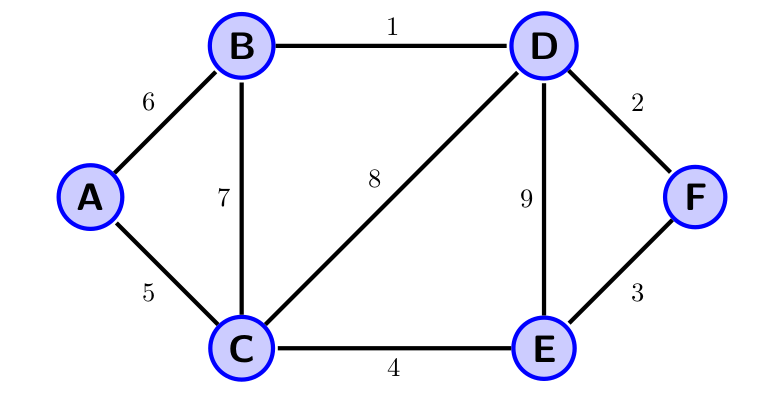
\includegraphics[width=\linewidth]{./images/dijkastra_01.png}
	\caption{Grafo com custos}
	\label{fig:dijkastra_graph}
  \end{minipage}
  \hfill
  \begin{minipage}[c]{0.58\linewidth}
	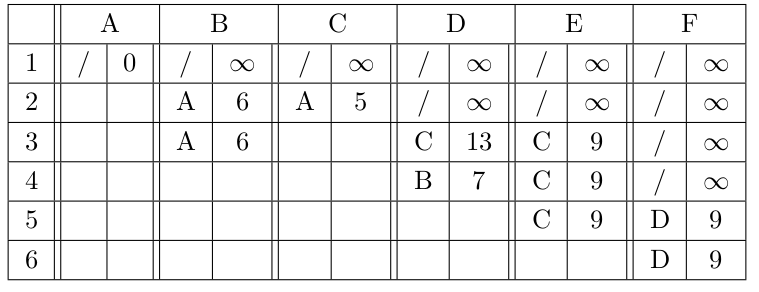
\includegraphics[width=\linewidth]{./images/dijkastra_02.png}
	\caption{Iterações do algoritmo Dijkastra}
	\label{fig:dijkastra_table}
  \end{minipage}
\end{figure}


\section{Definição do Problema} \label{sec:problem}

Para delimitar o escopo do problema, primeiro: elementos ativos não serão
considerados (ex.: terminal de linha óptico); segundo: uma fibra será
considerada ocupada (isto é, alocada) caso haja um comprimento de onda
associado a ela, ao longo desse artigo, vamos considerar apenas um comprimento
de onda por alocação (multiplexaćão por divisão de onda não será considerado);
terceiro: desconsidera-se atenuação; quarto: desconsidera-se o uso de
splitters, onde um mesmo comprimento de onda em uma fibra é "espalhado" para
$n$ fibras em um nó.

Fazendo um palalelo com \cite{artigorwa} e \cite{zang2000review}, podemos notar
a menção de "conversores ópticos", em uma aplicaćão mais genérica. O presente
artigo é um "subconjunto" do tema de alocação e roteamento de onda tratado nas
referências citadas.

- como uma rede nova é ocupada? De cima para baixo, ou de baixo para cima?
- qual seria a solução ótima?
- cabo de x para n para x fibras (fazer uma figura?);
- fatorial das combinações;
- tubos abertos vs. sangria;
- quando fazer manobras;
- fazer comparativo com o problema de otimização de fluxo máximo;

Considere uma rede óptica modelada como um grafo $G=(V,E)$,
onde $V$ representa os nós (caixas de emenda ou atendimento) e $E$ representa enlaces (cabos/fibras).
Cada aresta $e \in E$ possui um peso $w(e)$ correspondente ao custo físico (distância, atenuação ou custo de implantação).
O objetivo é determinar o caminho de menor custo entre um nó origem $s$ e um nó destino $t$.

\section{Desenvolvimento} \label{sec:algorithm}

O algoritmo de Dijkstra é empregado para resolver o problema.
O pseudo-código é dado a seguir:

\begin{enumerate}
    \item Inicializar todos os nós com distância infinita, exceto o nó origem $s$ que recebe 0.
    \item Marcar todos os nós como não visitados.
    \item Selecionar o nó não visitado com menor distância atual.
    \item Atualizar as distâncias dos vizinhos, se o novo caminho for mais curto.
    \item Repetir até que todos os nós tenham sido visitados ou que o destino $t$ tenha sido alcançado.
\end{enumerate}

...

\section{Conclusão}

Este artigo apresentou uma abordagem para o roteamento físico em redes ópticas
utilizando o algoritmo de Dijkstra. A fundamentação teórica mostrou a
relevância de representar redes como grafos ponderados e a comparação com
outros algoritmos. Ainda que problemas de roteamento óptico pertençam à classe
NP-difícil em sua formulação completa (com restrições de alocação de banda e
espectro), heurísticas como Dijkstra permitem soluções práticas e eficientes.
Como trabalhos futuros, recomenda-se a incorporação de restrições adicionais
(capacidade, espectro, múltiplos caminhos redundantes) e a aplicação de
técnicas híbridas com programação linear inteira para otimização global.


\bibliographystyle{./util/sbc}
\bibliography{./util/references}
\end{document}
